% ****** Start of file apssamp.tex ******
%
%   This file is part of the APS files in the REVTeX 4.2 distribution.
%   Version 4.2a of REVTeX, December 2014
%
%   Copyright (c) 2014 The American Physical Society.
%
%   See the REVTeX 4 README file for restrictions and more information.
%
% TeX'ing this file requires that you have AMS-LaTeX 2.0 installed
% as well as the rest of the prerequisites for REVTeX 4.2
%
% See the REVTeX 4 README file
% It also requires running BibTeX. The commands are as follows:
%
%  1)  latex apssamp.tex
%  2)  bibtex apssamp
%  3)  latex apssamp.tex
%  4)  latex apssamp.tex
%
\documentclass[%
 reprint,
%superscriptaddress,
%groupedaddress,
%unsortedaddress,
%runinaddress,
%frontmatterverbose, 
%preprint,
%preprintnumbers,
%nofootinbib,
%nobibnotes,
%bibnotes,
 amsmath,amssymb,
 aps,
%pra,
%prb,
%rmp,
%prstab,
%prstper,
%floatfix,
]{revtex4-2}

\usepackage[draft]{graphicx}% Include figure files
\graphicspath{images}
\usepackage{dcolumn}% Align table columns on decimal point
\usepackage{bm}% bold math
\usepackage{color}
\usepackage{acronym}
\usepackage{comment}
\usepackage{standalone}
\usepackage{tikz}
\usepackage{caption}
\usepackage{subcaption}
\usepackage{amssymb}
\usepackage{pifont}
%\usepackage{hyperref}% add hypertext capabilities
%\usepackage[mathlines]{lineno}% Enable numbering of text and display math
%\linenumbers\relax % Commence numbering lines

%\usepackage[showframe,%Uncomment any one of the following lines to test 
%%scale=0.7, marginratio={1:1, 2:3}, ignoreall,% default settings
%%text={7in,10in},centering,
%%margin=1.5in,
%%total={6.5in,8.75in}, top=1.2in, left=0.9in, includefoot,
%%height=10in,a5paper,hmargin={3cm,0.8in},
%]{geometry}

\newcommand{\jordan}[1]{\textbf{\textcolor{red}{JORDAN: #1}}}
\newcommand{\siong}[1]{\textbf{\textcolor{blue}{SIONG: #1}}}
\newcommand{\chris}[1]{\textbf{\textcolor{green}{CHRIS: #1}}}
\newcommand{\michael}[1]{\textbf{\textcolor{orange}{MICHAEL: #1}}}

\begin{document}

\preprint{APS/123-QED}

\title{Generalised gravitational burst searches with Generative Adverserial
Networks~\chris{Need to change the title if we don't search}}% Force line breaks with \\
\thanks{A footnote to the article title}%

%\author{Jordan McGinn, Chris Messenger, Ik Siong Heng}
 \altaffiliation[Also at ]{Physics Department, XYZ University.}%Lines break automatically or can be forced with \\

 \email{}
\affiliation{%
School of Physics \& Astronomy\\
University of Glasgow \\
Glasgow G12 8QQ, United Kingdom
}%


\date{\today}% It is always \today, today,
             %  but any date may be explicitly specified

\begin{abstract}
As the field of gravitational wave astronomy expands and as detectors become
more sensitive, there is a need for fast and efficient detection of various
sources. Gravitational wave bursts are a family of signals that remain
unmodeled, therefore, they have a low detection sensitivity to standard
detection schemes. This report examines the use of Generative Adversarial
Networks as a detection pipeline for gravitational wave burst signals. BurstGAN
is trained to detect three classes of burst signals: sine-Gaussian, Ring-downs
and white-noise bursts contained in white Gaussian noise. The resulting
sensitivity curves show that sine-Gaussian and Ring-downs are confidently
detectable at SNRs > while white-noise bursts require SNRs of >.~\chris{we'll
fix the abstract at the end}
%\begin{description} \item[Usage] Secondary publications and information
%retrieval purposes.  \item[Structure] You may use the \texttt{description}
%environment to structure your abstract; use the optional argument of the
%\verb+\item+ command to give the category of each item.  \end{description}
\end{abstract}

%\keywords{Suggested keywords}%Use showkeys class option if keyword
                              %display desired
\maketitle

%\tableofcontents

%%%%%%%%%%%%%%%%%%%%%%%%%%%%%%%%%%%%%%%%%%%%%%%%%%%%%%%%%%%%%%%%%%%%%%%%%%%%%%
\section{Introduction}
%%%%%%%%%%%%%%%%%%%%%%%%%%%%%%%%%%%%%%%%%%%%%%%%%%%%%%%%%%%%%%%%%%%%%%%%%%%%%%

\begin{comment}

\begin{itemize}
\item Need to introduce GWs - the current state of the field e.g. detections
and LVC papers
\item Introduce burst searches - what's the point of burst searches - lots of references
\item Discuss the family of burst waveforms currently used and why - not in detail, just
an introduction
\item Introduce ML techniques in GWs - lots of references
\item What this paper does on GANs in 1 paragraph
\item Describe the structure of the paper 
\end{itemize}
\end{comment}

Gravitational-wave (GW) astronomy is now an established field, starting with the first detection of a binary black hole merger \cite{} on September 2015. Following this, the first and second observations runs (O1 and O2) of Advanced LIGO and Advanced Virgo reported several more mergers \cite{}. On August 2017 a binary neutron star merger was observed alongside its electron-magnetic counterpart for the first time, giving rise to multimessenger gravitational wave astronomy. 

GW bursts are transient signals of typically short duration ($<$ 1s) whose waveforms are not accurately modelled or are complex to re-produce. Astrophysical sources for such transients include: \jordan{should i include a list of these?}. Since GW bursts are un-modelled they are not sensitive to template based detection schemes such as matched-filtering \cite{}, instead, detection involves distinguishing the signal from detector noise. This is only possible if the detector noise is well characterised and the candidate signal can be differentiated from system or environmental glitches. As such, GW burst searches rely on an astrophysical burst signature appearing in multiple detectors. \jordan{how deep should i go? with coherent WaveBurst etc?}

Many GW burst algorithms \cite{cite the shit outta this} are tested and tuned using model waveforms that may or may not have astrophysical significance but have easy to define parameters and share characteristics of real bursts that is enough to simulate coincident non-stationary deviations between detectors. Such waveforms may have long-duration, short bandwidth (ringdowns), long-duration, large bandwidth (inspirals) and many algorithms make use of sine-Gaussians: a Gaussian modulated sine wave that is characterised by it's central frequency and narrow bandwidth. This makes it a great tool for diagnosing LIGOs sensitivity to frequency. 

We aim to explore the use of machine learning in generating and interpreting these mock GW burst signals. Neural networks have shown to replicate the sensitivities of matched filtering in GW detection \cite{} and rapid parameter estimation \cite{}, however these methods have primarily been focused on binary black hole signals and have not yet expanded to burst examples. A subset of deep learning that has seen fruitful development in recent years \cite{} is Generative Adversarial Networks (GANs). These unsupervised algorithms learn patterns in a given training data set using an adversarial process. The generations from GANs are state-of-the-art in fields such as high quality image fidelity, image and text-to-image translation and video prediciton \cite{} and there is notable works on time series generations /cite. 





\begin{comment}
The detections of gravitational waves by Advanced Laser Interferometer
Gravitational wave Observatory (aLIGO) and Advanced Virgo [1–5], have opened up
new avenues to explore the Universe. Astrophysical sources of transient
gravitational waves include the merging of compact binary star systems like
black holes and/or neutron stars [6], core-collapse supernova [7], pulsar
glitches [8] and other events involving accelerating massive objects.
Gravitational wave bursts (GWBs) are an exciting area of research as the
emissions process of such waves is not well understood. The waveforms often
depend on complicated orbital dynamics and equations of state which limit the
sensitivity on searching for burst sources. Typically, the duration of burst
signals are short with amplitudes that can be greater than the detector noise.
Burst searches look for excess power contained in a time-frequency plot and
rely on consistent arrival times, waveform shapes and frequencies between
detectors. We focus on utilising an unsupervised form of machine learning
called Generative Adversarial Networks [9] as a generalised GW transient
search. A two detector case is considered such that the signals retain their
form between detections and a defined time delay between detections relating to
the sky orientation of the source.
\end{comment}

%%%%%%%%%%%%%%%%%%%%%%%%%%%%%%%%%%%%%%%%%%%%%%%%%%%%%%%%%%%%%%%%%%%%%%%%%%%%%%
\section{Generative Adversarial Networks}
%%%%%%%%%%%%%%%%%%%%%%%%%%%%%%%%%%%%%%%%%%%%%%%%%%%%%%%%%%%%%%%%%%%%%%%%%%%%%%

\begin{comment}
\begin{itemize}
\item Describe GANs in detail but really focus on the fact that the reader is a
GW data analyst - not a computer scientist
\item A diagram would be very useful
\item Do not discuss our specific case here - just stay general
\item A subsection on the specific advanced flavour of GAN that you are using
here - motivate this choice.
\end{itemize}
\end{comment}

\begin{figure}
    \centering
    \begin{subfigure}[t]{0.45\columnwidth}
        \centering
        %\documentclass{article}
%\usepackage{comment}
%\usepackage{tikz}
%\usetikzlibrary{shapes.geometric, arrows, calc}

%\begin{document}
    
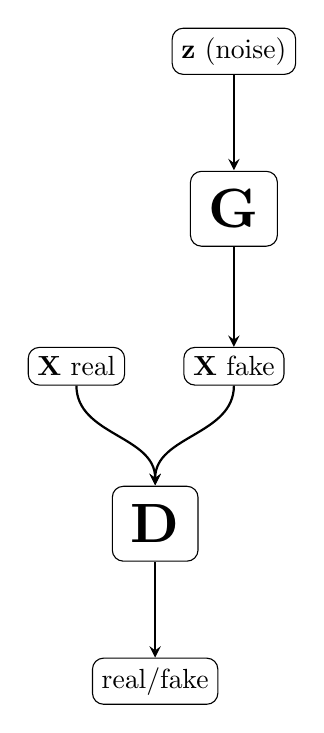
\begin{tikzpicture}[node distance=2cm]

\tikzstyle{zinput} = [rectangle, rounded corners, text centered, draw=black]%, fill=red!30]
\tikzstyle{generator} = [rectangle, rounded corners, text centered, draw=black]%, fill=red!30]
\tikzstyle{X real} = [rectangle, rounded corners, text centered, draw=black]%, fill=red!30]
\tikzstyle{X fake} = [rectangle, rounded corners, text centered, draw=black]%, fill=red!30]
\tikzstyle{X real} = [rectangle, rounded corners, text centered, draw=black]%, fill=red!30]
\tikzstyle{discriminator} = [rectangle, rounded corners, text centered, draw=black]%, fill=red!30]
\tikzstyle{real/fake} = [rectangle, rounded corners, text centered, draw=black]%, fill=red!30]

\tikzstyle{arrow} = [thick,->,>=stealth]

\node (r) [X real] {\textbf{X} real};
\node (f) [X fake, right of = r] {\textbf{X} fake};
\node (G) [generator,above of = f, scale = 2] {\textbf{G}};
\node (z) [zinput] [zinput, above of = G] {\textbf{z} (noise)};
\node (D) [discriminator, below of = f, xshift = -1cm, scale = 2] {\textbf{D}};
\node (rf) [real/fake, below of = D] {real/fake};

\draw [arrow] (z) -- (G);
\draw [arrow] (G) -- (f);
\draw [arrow] (r) edge[out=270,in=90] (D);
\draw [arrow] (f) edge[out=270,in=90] (D);
\draw [arrow] (D) -- (rf);

\end{tikzpicture}
%\end{document}
%     without .tex extension
        \caption{Vanilla GAN}
        \label{fig:GAN}
    \end{subfigure}\hfill
    \begin{subfigure}[t]{0.55\columnwidth}
        \centering
        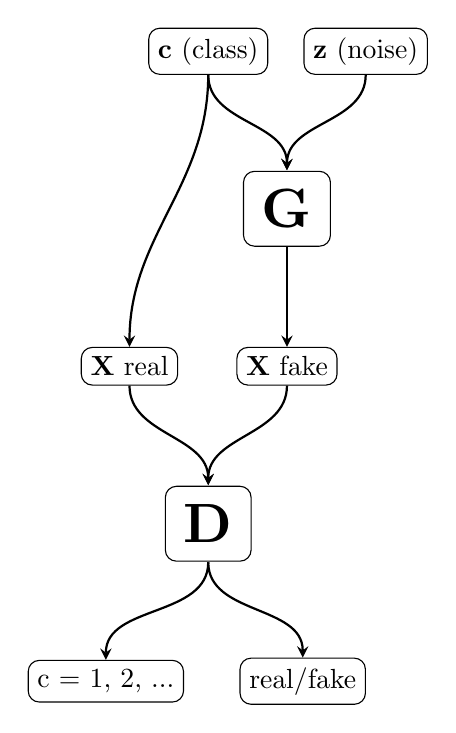
\begin{tikzpicture}[node distance=2cm]

\tikzstyle{zinput} = [rectangle, rounded corners, text centered, draw=black]%, fill=red!30]
\tikzstyle{generator} = [rectangle, rounded corners, text centered, draw=black]%, fill=red!30]
\tikzstyle{X real} = [rectangle, rounded corners, text centered, draw=black]%, fill=red!30]
\tikzstyle{X fake} = [rectangle, rounded corners, text centered, draw=black]%, fill=red!30]
\tikzstyle{X real} = [rectangle, rounded corners, text centered, draw=black]%, fill=red!30]
\tikzstyle{discriminator} = [rectangle, rounded corners, text centered, draw=black]%, fill=red!30]
\tikzstyle{real/fake} = [rectangle, rounded corners, text centered, draw=black]%, fill=red!30]
\tikzstyle{coutput} = [rectangle, rounded corners, text centered, draw=black]%, fill=red!30]

\tikzstyle{arrow} = [thick,->,>=stealth]

\node (r) [X real] {\textbf{X} real};
\node (f) [X fake, right of = r] {\textbf{X} fake};
\node (G) [generator,above of = f, scale = 2] {\textbf{G}};
\node (z) [zinput] [zinput, above of = G, xshift = 1cm] {\textbf{z} (noise)};
\node (c) [coutput, left of = z] {\textbf{c} (class)};
\node (D) [discriminator, below of = f, xshift = -1cm, scale = 2] {\textbf{D}};
\node (rf) [real/fake, below of = D, xshift = 1.2cm] {real/fake};
\node (co) [coutput, left of = rf, xshift = -0.5cm] {c = 1, 2, ...};

\draw [arrow] (z) edge[out=270,in=90] (G);
\draw [arrow] (c) edge[out=270,in=90] (G);
\draw [arrow] (c) edge[out=270,in=90] (r);
\draw [arrow] (G) -- (f);
\draw [arrow] (r) edge[out=270,in=90] (D);
\draw [arrow] (f) edge[out=270,in=90] (D);
\draw [arrow] (D) edge[out=270,in=90] (rf);
\draw [arrow] (D) edge[out=270,in=90] (co);

\end{tikzpicture}%     without .tex extension
        \caption{AC-GAN}
        \label{fig:ACGAN}
    \end{subfigure}\hfill
    \caption{Comparison of the original GAN method and the Auxiliary Conditional-GAN method }
\end{figure}

Generative adversarial networks (GANs) have seen considerable success in recent
years as a generative machine learning model. GANs work to train two competing
neural networks, consisting of a discriminator \textbf{D} that is trained to distinguish
between real and fake data and a generator \textbf{G} that produces synthetic
reproductions of the real data. The GAN method has \textbf{G} perform a mapping
from an input noise vector \textbf{z} to its representation of the data and \textbf{D} maps its
input \textbf{x} to a probability that the input came form either the training
data or \textbf{G}.  During training, \textbf{D} is given a batch of samples that contains one half real data (labelled as 1)
and one half fake data (labelled as 0) which it then makes predictions on. The
loss for \textbf{D} is calculated by comparing its predictions to the labelled data through the binary cross-entropy function. The training process
of a GAN alternatively updates the weights of the \textbf{D} and \textbf{G} based on information
on its competitors loss function. This loss of \textbf{D} is used to update the weights
of \textbf{G} to produce more realistic samples of the input distribution, the loss of G
encourages \textbf{D} to update its classification abilities. Both networks compete
in a minimax game that is tied to a value function V (D, G) which \textbf{G} is trying
minimise and \textbf{D} is trying to maximise:

\begin{multline}
\mathop{\text{min}}_{G}  \mathop{\text{max}}_{D} V(D,G) = \mathbb{E}_{\bold{x} \sim p_{\text{r}}(\bold{x})} [\text{log} D(\bold{x})] \\ + \mathbb{E}_{\bold{z} \sim p_{\text{z}}(\bold{z})} [\text{log}(1-D(G(\bold{z})))]
\label{equation:GANloss}
\end{multline}
\subsection{Auxiliary conditional GANs}
In theory this will eventually lead to the local Nash equilibrium [18] where
both neural networks are trained optimally. In practice, however, GANs are
notoriously difficult to train. Such difficulties include: Non-convergence,
where the model parameters oscillate and the loss never converges. Mode
collapse where G produces a limited diversity of samples, and the diminishing
gradient problem when applying gradient descent to a
non-continuous function.  \\ To overcome some of these difficulties [blank]
proposed adding structure to the latent space by providing G with a class
label. This has the effect of making a point in latent space conditional on a
provided class. [blank] extends this idea further by requiring D to output a
probability of the data belonging to each class. 

%%%%%%%%%%%%%%%%%%%%%%%%%%%%%%%%%%%%%%%%%%%%%%%%%%%%%%%%%%%%%%%%%%%%%%%%%%%%%%
\section{Method}
%%%%%%%%%%%%%%%%%%%%%%%%%%%%%%%%%%%%%%%%%%%%%%%%%%%%%%%%%%%%%%%%%%%%%%%%%%%%%%

\begin{itemize}
\item Need to introduce the scheme you propose to use
\item A paragraph or subsection on the data generation being very clear on all
5 waveform models and the prior parameter space for each
\item A subsection on the design of the network architecture
\item A subsection on the "box" and why we implement it
\item A subsection on the training of the network - give rough timings and rule
of thumb decisions made
\item Do not discuss the results here 
\end{itemize}

To simulate gravitational burst sources, three GW signal morphologies, spanning a range of frequencies, duration and time delays were tested. The three families are:\\

time delay/antenna pattern/lalsuite etc \\

archetecture/hyperparameters

%%%%%%%%%%%%%%%%%%%%%%%%%%%%%%%%%%%%%%%%%%%%%%%%%%%%%%%%%%%%%%%%%%%%%%%%%%%%%%
\section{Results}
%%%%%%%%%%%%%%%%%%%%%%%%%%%%%%%%%%%%%%%%%%%%%%%%%%%%%%%%%%%%%%%%%%%%%%%%%%%%%%

\begin{itemize}
\item Begin by outlining the type of results you will be presenting
\item A subsection on the general quality of generated waveforms - we may need
to have overlaps between generated wavefoms and training data (maybe)
\item A subsection on the descriminator - maybe a confusion matrix?
\item a subsection on the latent space varaition within each class - fixed
class, sliding in latent space.
\item A subsection on the class space variation - fixed latent space and
sliding in the class space.
\item A final subsection on the general waveform model based on random latent
and class space locations.
\item Make no conclusions.
\end{itemize}

\begin{figure}
    \centering
    \includegraphics[scale=0.1]{images/real_fake_sample.png}
    \caption{Caption}
    \label{fig:my_label}
\end{figure}


%%%%%%%%%%%%%%%%%%%%%%%%%%%%%%%%%%%%%%%%%%%%%%%%%%%%%%%%%%%%%%%%%%%%%%%%%%%%%%
\section{Conclusions}
%%%%%%%%%%%%%%%%%%%%%%%%%%%%%%%%%%%%%%%%%%%%%%%%%%%%%%%%%%%%%%%%%%%%%%%%%%%%%%

\begin{itemize}
\item Summarise the paper
\item Dedicate a paragraph to each of the key results discussed in the previous
section
\item Have at least one paragraph on the future directions of this work
\item Conclude with a positive paragrpah about the potential uses and impact of
the approach.
\end{itemize}

\bibliography{apssamp}% Produces the bibliography via BibTeX.

\Appendix

\begin{table*}[t]
\begin{center}
\begin{tabular}{ r  l  l  l  l  l  l}  
 \hline
 Operation & Kernel & Strides & Output Shape & BN & Dropout & Activation \\ 
 \hline
 G(\textbf{z}): Input \textbf{z} $\sim$ Normal(0,0.02) & N/A & N/A & (100,) & \ding{55} & 0 & N/A \\  
 Dense & N/A & N/A & (32768,) & \ding{55} & 0 & ReLU \\  
 Class input c & N/A & N/A & (1,) & \ding{55} & 0 & N/A \\
 Embedding & N/A & N/A & (1, 120) & \ding{55} & 0 & N/A \\
 Dense & N/A & N/A & (1,128) & \ding{55} & 0 & ReLU \\ 
 Reshape \textbf{z} & N/A & N/A & (128, 256) & \ding{55} & 0 & N/A \\
 Reshape c & N/A & N/A & (128, 1) & \ding{55} & 0 & N/A \\
 Concatenate & N/A & N/A & (128, 257) & \ding{55} & 0 & N/A \\
 Reshape & N/A & N/A & (64, 514) & \ding{55} & 0 & N/A \\
 Transposed Convolution & 18x1 & 2 & (256, 256) & \ding{51} & 0 & ReLU\\
 Transposed Convolution & 18x1 & 2 & (512, 128) & \ding{55} & 0 & ReLU\\
 Transposed Convolution & 18x1 & 2 & (1024, 64) & \ding{55} & 0 & ReLU\\
 Convolution & 18x1 & 1 & (1024, 1) & \ding{55} & 0 & Tanh \\
 Sky input & N/A & N/A & (3,) & \ding{55} & 0 & N/A \\
 Concatenate & N/A & N/A & (1027,) &  \ding{55} & 0 & N/A \\
 Lambda & N/A & N/A & (1024, 2) & \ding{55} & 0 & N/A \\
 D(\textbf{x}): Input \textbf{x} & N/A & N/A & (1024, 2) & \ding{55} & 0 & N/A \\
 Convolution & 14x1 & 2 & (512, 64) & \ding{55} & 0.5 & Leaky ReLU \\
 Convolution & 14x1 & 2 & (256, 128) & \ding{55} & 0.5 & Leaky ReLU \\
 Convolution & 14x1 & 2 & (128, 256) & \ding{55} & 0.5 & Leaky ReLU \\
 Convolution & 14x1 & 2 & (64, 512) & \ding{55} & 0.5 & Leaky ReLU \\
 Flatten & N/A & N/A & (32768,) & \ding{55} & 0 & N/A \\
 Dense & N/A & N/A & (1,) & \ding{55} & 0 & Sigmoid \\
 Dense & N/A & N/A & (5,) & \ding{55} & 0 & Softmax \\
 \hline
 Optimizer & \multicolumn{6}{l}{Adam($\alpha$ = 0.0002, $\beta_{1}$ = 0.5)} \\
 Batch size & \multicolumn{6}{l}{100}  \\
 Iterations & \multicolumn{6}{l}{60000}  \\
 Leaky ReLU slope & \multicolumn{6}{l}{0.2} \\
 Weight initialization & \multicolumn{6}{l}{Gaussian($\mu$ = 0, $\sigma$ = 0.02)} \\
 Generator loss & \multicolumn{6}{l}{Binary cross-entropy} \\
 Discriminator loss & \multicolumn{6}{l}{Binary cross-entropy \& sparse categorical cross-entropy} \\ 
 \hline
\end{tabular}
\end{center}
\end{table*}

\end{document}
%
% ****** End of file apssamp.tex ******
